%! TeX Program = LuaLaTeX

\documentclass{ltjsarticle}
%\documentclass[
%    paper = a4paper,
%    fontsize = 12Q,
%    jafontsize = 12Q,
%    %line_length = ?zw,
%    %number_of_lines = ?,
%    article
%]{jlreq}

\usepackage{graphicx}

\usepackage[match]{luatexja-fontspec}
\setmainfont{Linux Libertine O}
\setmainjfont{Source Han Serif SC}[Language = Chinese Simplified, YokoFeatures = {JFM = eva/{smpl, nstd}}]
\setsansfont{Linux Biolinum O}
%\setsansjfont{Source Han Sans SC}[Language = Chinese Simplified, YokoFeatures = {JFM = eva/{smpl, nstd}}]
\setmonofont[Scale=MatchLowercase, FakeStretch=1.137121, RawFeature=-notdef]{Iosevka Slab}
%\setmonojfont{Source Han Sans SC}

\usepackage{luatexja-adjust}
\ltjenableadjust[priority = true]

\usepackage{listings}
%\lstloadlanguages{TeX}
\lstset{
    %language = TeX,
    basicstyle = \ttfamily\small,
    breaklines = true,
    columns = flexible,
    numbers = left,
    numberstyle = \tiny,
    stepnumber = 1,
    gobble = 4,
    numbersep = 6pt,
    escapechar = §
}

\usepackage{hyperref}
\hypersetup{
    hidelinks,
    pdftitle = {Evangelion-JFM},
    pdfauthor = {RadioNoiseE},
    pdfsubject = {TeX},
    pdfkeywords = {Japanese Font Metric},
    pdfstartview = FitV
}

\long\def\feature#1#2#3{{\vskip8pt\vbox{\normalsize\parindent=\zw\hangindent=2\zw\texttt{#1 --> ({\itshape #2\/})}\\\indent#3\par}}}
\def\meta#1{{\normalfont\rmfamily\itshape$\langle$#1\/$\rangle$}}
\def\空{\quad}
\def\段{\par}
\def\LuaTeX{Lua\kern-.2ex\TeX}
\def\pTeX{p\kern-.2ex\TeX}
\def\pdfTeX{pdf\TeX}

\title{\sffamily\bfseries Evangelion Japanese Font Metric for \LuaTeX}
\author{\large \url{https://github.com/RadioNoiseE/Evangelion-JFM}}
\date{西历2023年}

\begin{document}
\parindent=2\zw\parskip=2pt

\maketitle

\begin{abstract}
    本文档将介绍名为Evangelion Japanese Font Metric(下简称为``\textsf{Eva-JFM}'')的JFM文件。其适用于简体中文(以下简称为「简中」)、繁体中文(以下简称为「繁中」)及日文字体的横直排。旨在提供一个充分利用\LuaTeX{}-ja的\texttt{priority}特性,基于标准\cite{jlreq}的同时,支持一些罕用特性的JFM文件。文档暂仅使用中文撰写。\段
    % This document introduces a JFM file named ``Evangelion-JFM'' (hereinafter referred to as ``\textsf{Eva-JFM}''). It supports vertical and horizontal written Simplified Chinese (hereinafter referred to as ``SC''), Traditional Chinese (hereinafter referred to as ``TC''), and Japanese (hereinafter referred to ad ``JP''). It aims to provide a JFM file that takes full advantage of the \texttt{priority} and other powerful features from \LuaTeX{}-ja, supporting the widely accepted standards (i.e. \cite{jlreq}), and supporting some rarely-used features. The documentation is written in both Chinese Simplified and English.
\end{abstract}

\section{背景及略介:Background Knowledge and a Rough Introduction}
\TeX{}是高德纳教授于20世纪末开发的强大排版引擎,能够完全满足西文排版的需求。然因时代局限性\footnote{如没有事实上的统一字符编码等。}以及客观原因\footnote{如中日字符集较大,以及书写方式的不同(纵书、横书),标点等。}对中日排版支持十分有限。为达成中日排版需求,在宏扩展(如\textsf{CJK}等)之外出现了引擎扩展。影响力较大的是\pTeX{}系列。\段
\pTeX{}系列采用虚拟字体的理念,使用\texttt{TFM/VF}映射TrueType或OpenType字体完成排版。其不支持宏配置字体,也不支持直接生成PDF格式文件。但可以满足日本的传统横纵排版需求(工业标准)。\段
\pdfTeX{}则是当时另一个\TeX{}的引擎扩展,支持不经DVI格式直接输出PDF格式的文件。然对Unicode(字符编码)及TrueType、OpenType(「现代」矢量字体格式)的支持繁琐或有限。\LuaTeX{}便是基于\pdfTeX{}的引擎扩展,在原生支持Unicode下提供Lua语言扩展(使能够使用\textsf{fontloader}等模块)支持现代字体。宏配置字体特性由\textsf{luaotfload}宏集提供。它也支持直接生成PDF文件。\段
\LuaTeX{}-ja可看作是对两者的合并。这是一个由日本开发者北川弘典首倡的\LuaTeX{}下的日文支持项目,即将\pTeX{}(大部分)移植到\LuaTeX{}下。由于\LuaTeX{}支持宏配置字体,故不需要\texttt{VF}文件为字体提供映射,但为标点挤压等需求保留并扩展\footnote{如优先挤压(\texttt{priority})特性,及一些特殊字符(如\texttt{parbdd}、\texttt{glue})等。}了JFM文件。\段
本项目就是一个JFM文件。使用\LuaTeX{}的\texttt{callback},将简中、繁中、日文及横纵方向、行间标点、悬挂标点、压缩字体等特性集中于\texttt{jfm-eva.lua}单个文件中。用户可按需调用特性来完成高质量的中日排版。

\section{安裝及本地配置:Installation and Local Configs}
本项目将源文件托管于GitHub平台,暂未上传至Comprehensive \TeX{} Archive Net(CTAN)。用户可使用
\begin{lstlisting}
    mkdir Evangelion-JFM [&&] cd Evangelion-JFM
    git clone https://github.com/RadioNoiseE/Evangelion-JFM
\end{lstlisting}
获取源文件,再将其放置在本地的\texttt{TEXMF}路径中,如
\begin{lstlisting}
    ~/Library/texlive/2023/texmf-dist/tex/luatex/eva-jfm
\end{lstlisting}
等。最后运行
\begin{lstlisting}
    mktexlsr
\end{lstlisting}
更新本地\TeX{}的\texttt{Ls-R}文件即可。\段
本文件一般情况下无需用户进行本地配置,但若有特殊需求可见第\ref{sec:config}节。

\section{使用:Using}
以下是在\LaTeX{}下使用繁中字体进行直排的示例
\begin{lstlisting}
    \usepackage{luatexja-fontspec, luatexja-adjust}
    \setmainjfont{Source Han Serif TC}[Language = Chinese Traditional, TateFeatures = {JFM = eva/{vert, trad, nstd}}]
    \ltjenableadjust[priority = true]
\end{lstlisting}
(注意需要调用支持直书的文档类或使用\texttt{\string\tate}命令)。\LuaTeX-ja的JFM语法为:
\begin{lstlisting}
    jfm = §\meta{JFM name}§/{§\meta{JFM features}§}
\end{lstlisting}
而一般情况使用\texttt{\string\setmainjfont}时则为:
\begin{lstlisting}
    \setmainjfont{§\meta{font name}§}[Language = §\meta{language name}§, §\meta{dir}§ = {JFM = §\meta{JFM name}§/{§\meta{JFM features}§}}]
\end{lstlisting}
其中,\meta{font name}自然为需要的字体名称。\meta{language name}在使用日文字体时可忽略,而使用简中、繁中字体时为必填,因\LuaTeX-ja会默认将其覆盖为\texttt{Japanese}选项,而这会带来灾难性的后果\footnote{比如错误的标点位置:日文为冒号及分号中置、其余偏靠,简中是全部偏靠,而繁中则是统统中置。}。\meta{dir}选填\texttt{TateFeatures}(直书)或\texttt{YokoFeatures}(横书)。其后的\meta{JFM name}为调用JFM的文件名\footnote{\LuaTeX-ja会依\texttt{jfm-\meta{JFM name}.lua}的格式来查找该文件。}。最后的\meta{JFM features}选项为选择使用的JFM特性,详细请看第\ref{sec:feat}章。\段
其他情况下设置JFM及其更多信息请看\LuaTeX-ja文档\cite{luatexja-doc}。

\section{支持特性:Supported Features}\label{sec:feat}
本章节将介绍\textsf{Eva-JFM}的所有特性,分别为:语言特性、方向特性、扩展特性及私有特性。

\subsection{語言特性:Language Features}
本区特性必填且只可填一个。不然则会报错。\段
\feature{jp}{JaPanese}{%
    日本语特性。当使用日文字体时需调用该特性。其与简中、繁中区别在于问号及感叹号后插入的伸缩胶量。影响特性\texttt{lgp},且对内部分组有影响。
}
\feature{trad}{TRADitional chinese}{%
    繁中特性。当使用繁体中文字体时需调用。与简中、日本语特性的区别源于中置的标点。故,对于全部标点左右插入的伸缩胶的量都与简中、日本语不同。针对句点紧挨闭括号、标点位于句末时等皆有优化。
}
\feature{smpl}{SiMPLified}{%
    简中特性,使用简体中文字体排版时调用。与日本语、繁中特性区别源于分号及冒号等全部偏靠从而影响其左右插入伸缩胶的量。\textsf{Eva-JFM}对一些(不该出现的)神奇情况(如两个句号同时出现、开括号后出现问号等)进行优化。对问号、感叹号等作了特殊处理。
}

\subsection{方向特性:(Writing) Direction Features}
本分区特性与全部其他特性兼容,可同时调用。\段
\feature{vert}{VERTical writing}{%
    直书特性。对标点挤压、分组有影响。直书时必须调用。
}

\subsection{擴展特性:Extended Features}
本区特性\texttt{hgp}不依赖\texttt{vert}特性,其余需同\texttt{vert}特性同时调用。否则报错。\段
\feature{extd}{EXTenDed font}{%
    压缩字体特性。目前仅支持横比纵为100比80的字体压缩\footnotemark{}。需同\texttt{extend}(\textsf{luaotfload})或\texttt{FakeStretch}(\textsf{fontspec})同时使用。
}\footnotetext{日本新闻字体,如每日新闻明朝体。}
\feature{lgp}{LineGap Punctuations}{%
    行间标点特性。该特性将部分标点「悬挂」至行间。日文字体时与繁、简中字体时会有区别。详见第\ref{sec:lgp}章。
}
\feature{hgp}{HanGing Punctuations}{%
    悬挂标点特性。该特性将部分标点「悬挂」于行末。仅简中、日文字体拥有该特性。
}

\subsection{私有特性:Dark Features}
使用本区特性前请先确保你清楚地知道你在做什么。\段
\feature{nstd}{Non STandarD}{%
    忽略标准特性。字体排印标准\cite{jlreq}认为逗号的压缩权重应比句号要低。本特性将句号的压缩优先级与逗号交换,使逗号被优先压缩\footnotemark{}。仅在使用\textsf{luatexja-adjust}宏集时有效。
}\footnotetext{考虑逗号、句号在文字系统中占的重量,以及「开明」压缩风格。}

\section{行間標點特性:More About Linegap Punctuations}\label{sec:lgp}
本章节将提供更多详细的关于行间标点特性的信息,以及可能出现的问题及其解决方案。

\subsection{關於「懸掛」:About ``Hanging''}
行间标点可见于古籍之中,是将标点符号与直书结合妥协的产物。\段
传统上悬挂句号与逗号。而\textsf{Eva-JFM}特性在繁中、简中特性下会悬挂句号、逗号、顿号、冒号及分号,日文字体下则不悬挂冒号及分号。原因在于日本习惯上将冒号与分号看作「中点类」,直书时横置处理。\段
本JFM将全部标点悬挂于字体右下位置。详见下一节。

\subsection{懸掛的位置:Hanging Position}
%Figure Here
\begin{figure}[htb]
    \centering
    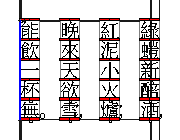
\includegraphics[height = 12\zh]{figure/fig-tc.pdf}\空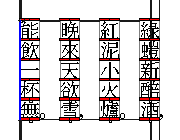
\includegraphics[height = 12\zh]{figure/fig-jp.pdf}
    \caption{行间标点特性示意图}\label{fig:lgp}
\end{figure}

标点悬挂的位置有以下考量,可参照图\ref{fig:lgp}。若有特殊需求请看第\ref{sec:config}节。优先级由上至下。
\begin{itemize}
    \item 三种字体风格统一,位置原则上一致(故,繁中字体也悬挂于右下、而非居中);
    \item 不同标点中的相同(似)元素位置相同;
    \item 繁中、简中、日文字体标点触字框右边线;
    \item 不同标点符号因形状不同可于字框底线略下沉或上浮;
    \item 不同标点符号因大小不同可靠近或远离字框右边线;
    \item 三种字体可分别因字符设计的差异而位置略微区别。
\end{itemize}

\subsection{用戶配置:Configurations}\label{sec:config}
本特性是以三套思源字体为基准设计的。而由于各字体的标点符号位置不可避免会有不同,故在某些特殊情况下会出现错位影响视觉效果的情况。或是单纯对原设定而言更偏好其他设定等原因,本节提供自定义及调整的两种方法。第一种较简单但可移植性较差,而第二种虽繁琐但一劳永逸。

\subsubsection{修改原程式碼:Changing Parameters}
在\textsf{Eva-JFM}中,控制行间标点的分区分别为
\begin{lstlisting}
    [101,2] ==> [1]; [201,2] ==> [2]; [301,2] ==> [3].
\end{lstlisting}
只需调整其中\texttt{left}和\texttt{down}键的值即可。其中\texttt{left}为向右移动,\texttt{down}为向下移动。
具体可参照第\ref{sec:impl}章。

\subsubsection{使用外掛符號字體:Using Seperate Punctuation Font}
该方法的原理就是使用特殊的仅包含(标点)符号的字体来替换原有字体中的标点符号,从而稳定其表现。符号字体可使用\url{https://github.com/Buernia/Zhudou-Sans}处的开源字体。其基于思源黑体,还添加了许多其他符号(但这里我们只会用到六个符号)及标点挤压等特性。\段
将其放入\texttt{TEXMF}并更新\texttt{Ls-R}文件后即可使用\LuaTeX-ja提供的\texttt{AltFont}键进行替换,例元:
\begin{lstlisting}
    \setmainjfont[
        Language = §\meta{language}§,
        TateFeatures = {
            JFM = eva/{vert, lgp, §\meta{language}§},
            AltFont = {
                {Range = "§\meta{utf-8 code}§, Font = §\meta{symbol font}§}
            }
        }
    ]{§\meta{main font}§}
\end{lstlisting}
其中首个\meta{language}可选填\texttt{Japanese}、\texttt{Chinese Traditional}或\texttt{Chinese Simplified},第二个则填语言特性分区的对应\texttt{jp}、\texttt{trad}及\texttt{smpl}特性。\meta{utf-8 code}则为需要替换的标点符号的Unicode编码,如需替换句号(ideographic full stop,\texttt{U+3002})则填\texttt{3002}\footnote{编码可至\url{https://www.unicode.org/charts/unihanrsindex.html}查询。}即可。
\meta{symbol font}以及\meta{main font}填符号字体名称、正文字体名称即可。具体语法及示例可看\cite{luatexja-doc}。

\section{启發:Inspiration}
\textsf{Eva-JFM}的内部分组受\texttt{min10.tfm} \cite{min10}的启发,支持的\texttt{priority}特性则取自阿部紀行氏的\texttt{jlreq.lua} \cite{ltxjlreq}文件。其余可见参考文献。

\begin{thebibliography}{99}
    \addcontentsline{toc}{section}{\refname}
    \bibitem{jlreq} W3C Japanese Layout Task Force~(ed). \newblock Requirements for Japanese Text Layout (W3C Working Group Note), 2022, 2023. \newblock \url{https://www.w3.org/TR/jlreq/}.
    \bibitem{luatexja-doc} \LuaTeX-jaプロジェクトチーム. \newblock \LuaTeX-jaパッケージ, 2022, 2023.
    \bibitem{unicode} The Unicode Consortium. \newblock The Unicode Standard Version 15.0 - Core Specification, 2022.
    \bibitem{tex-by-topic} Victor Eijkhout. \newblock \TeX{} by Topic, A \TeX nician's Reference, Addison-Wesley, 1992.
    \bibitem{min10} 乙部厳己. \newblock min10フォントについて. \newblock \url{http://argent.shinshu-u.ac.jp/~otobe/tex/files/min10.pdf}.
    \bibitem{ltxjlreq} Noriyuki Abe. \newblock Jlreq Document Class, 2022. \newblock \url{https://github.com/abenori/jlreq}.
\end{thebibliography}

\section*{程式碼:Implementation}\label{sec:impl}
以下为\texttt{jfm-eva.lua}文件内容,供参考。%及二次开发等。
\lstinputlisting{jfm-eva.lua}

\end{document}
